\begin{frame}[t]
\frametitle{Current state of phylogenetics}
    \vspace{-3mm}
    \uncover<2->{
    \begin{adjustwidth}{-3.1em}{-3.1em}
        \begin{itemize}
            \item<2-> \textbf{Limiting assumption:} Events are independent across the tree
            % \item<3-> We know this assumption is frequently violated
        \end{itemize}
    \end{adjustwidth}
    }
    

    \vspace{-5mm}

    \begin{onlyenv}<1-2>
    \begin{center}
        % \transwipe<2>[direction=0, duration=3]
        % \includegraphics<2>[width=\textwidth]{../images/mascot-tree.png}
        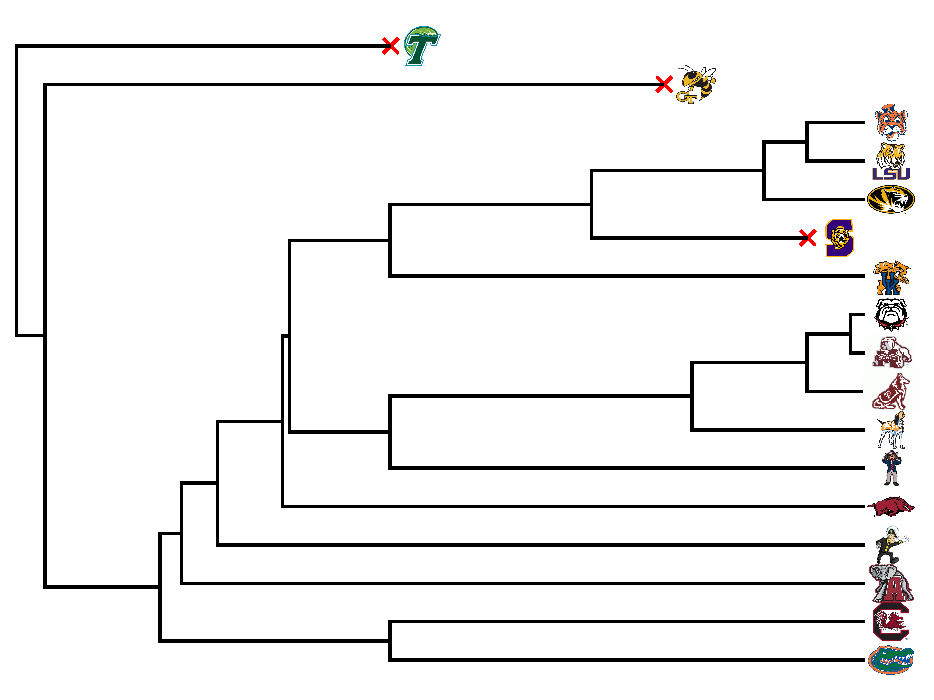
\includegraphics[width=\textwidth]{../mascot-tree/mascot-tree-shared.pdf}

    \end{center}
    \end{onlyenv}

    % \vspace{-1cm}
    \begin{onlyenv}<3->
    \begin{columns}
        \column{0.4\textwidth}
        \begin{minipage}[c]{\columnwidth}
        \begin{adjustwidth}{-2.1em}{}
        % \begin{onlyenv}<1-6>
        \begin{itemize}
            % \item<2-> Current phylogenetic methods assume events are independent 
            \item<3-> We know this assumption is frequently violated
            \item<5-> Why account for this non-independence?
            \begin{enumerate}
                \item<6-> Improve phylogenetic inference
                \item<7-> \textbf{Provide a general framework for inferring the
                        effect of community-scale processes on diversification}
            \end{enumerate}
        \end{itemize}
        % \end{onlyenv}
        \end{adjustwidth}
        \end{minipage}

        \column{0.6\textwidth}
        \begin{minipage}[t][\textheight][c]{\linewidth}
        \centerline{
        \includegraphics<3>[width=1.1\columnwidth]{../mascot-tree/mascot-tree-shared.pdf}
        \includegraphics<4->[width=1.1\columnwidth]{../mascot-tree/mascot-tree-shared-events.pdf}
        }
        \end{minipage}
    \end{columns}
    \end{onlyenv}
\end{frame}
